\documentclass[12pt, oneside, a4paper]{report}
\usepackage{hyperref,graphicx}
\usepackage[top=3cm, bottom=3cm, left=3cm, right=3cm]{geometry}
\usepackage{setspace}
\usepackage{fontspec}
\usepackage{float}
\usepackage{color}
\usepackage[usenames,dvipsnames,svgnames,table]{xcolor}
\usepackage{xunicode}
\usepackage{array}
\usepackage{booktabs,bookmark}
\usepackage{longtable}
\usepackage{ragged2e}
\usepackage[font={footnotesize,it}]{caption}
\usepackage{parskip}
\usepackage{amsmath}
\usepackage{amssymb}
\usepackage{bm}
\usepackage{textcomp}
%\usepackage[customcolors]{hf-tikz}
\usepackage{xspace}
\usepackage[Greek,Latin]{ucharclasses}
\usepackage{xltxtra}
\usepackage{xgreek} 
\usepackage[sort&compress,numbers]{natbib}
\usepackage{float}
\usepackage{mathtools}

% \usepackage[utf8]{inputenc}

%\usepackage{minted}

\renewcommand{\labelenumii}{\theenumii}
\renewcommand{\theenumii}{\theenumi.\arabic{enumii}.}

%\floatname{algorithm}{Αλγόριθμος}
\renewcommand\figurename{Εικόνα}
%\renewcommand\tablename{Πίνακας}

\setTransitionsForGreek{\setlanguage{greek}}{\setlanguage{american}} % Instead of american, any other language can be used

\renewcommand\thesection{\arabic{section}}

\hypersetup{
 %bookmarks=true, % show bookmarks bar?
unicode=true, % non-Latin characters in Acrobat’s bookmarks
pdftoolbar=true, % show Acrobat’s toolbar?
pdfmenubar=true, % show Acrobat’s menu?
pdffitwindow=false, % window fit to page when opened
pdfstartview={FitH}, % fits the width of the page to the window
pdftitle={Stakeholder's Requirements Specification}, % title
pdfauthor={Daphne Tsolissou}, % author
pdfsubject={}, % subject of the document
pdfcreator={LaTeX}, % creator of the document
% pdfproducer={LateX}, % producer of the document
%pdfkeywords= % list of keywords
pdfnewwindow=true, % links in new window
colorlinks=false, % false: boxed links; true: colored links
linkbordercolor={1 1 1}, % color of internal links (change box color with linkbordercolor)
%citecolor=white, % color of links to bibliography
citebordercolor={1 1 1},
filecolor=magenta, % color of file links
urlcolor=cyan % color of external links
}

\setmainfont{Times New Roman}
\singlespacing
\frenchspacing
\setlength{\parindent}{0.6cm}
\setlength{\parskip}{0.5pt}

\begin{document}
%      \parbox[l]{\textwidth}{
\flushleft{\Huge{\textbf{Έγγραφο απαιτήσεων εμπλεκομένων μερών (StRS)}}}\\
\flushleft{\Huge{\textbf{Stakeholders Requirements Specification}}}\\
\flushleft{\footnotesize{ΠΡΟΣΑΡΜΟΓΗ ΤΟΥ ΑΝΤΙΣΤΟΙΧΟΥ ΕΓΓΡΑΦΟΥ ΤΟΥ ΠΡΟΤΥΠΟΥ ISO/IEC/IEEE 29148:2011}}\\
    \vspace{1cm}
\flushleft{\Large{\textbf{Χρήστες Εθελοντές}}}\\
    \vspace{1cm}

\pagestyle{plain}
\pagenumbering{arabic}
\normalsize
\section{Εισαγωγή}

\subsection{Ταυτότητα-επιχειρησιακοί στόχοι}

\hspace{0.6cm}Βασικός στόχος της πλατφόρμας είναι να εξασφαλίσει στους χρήστες του έναν εύχρηστο και αξιόπιστο τρόπο ενημέρωσης πάνω στην μεγάλη αγορά των κινητών τηλεφώνων, παρέχοντας τις τοποθεσίες από τις οποίες μπορούν να τα προμηθευτούν αλλά και τις τιμές κάθε καταστήματος για το εκάστοτε προϊόν. Ταυτόχρονα θα παρέχει έναν βολικό τρόπο να καταγράφουν οι ίδιοι μία νέα τιμή που παρατήρησαν για κάποιο υπάρχον κινητό σε ένα καινούργιο κατάστημα ή να την ανανεώσουν σε ένα κατάστημα που υπάρχει. 

\hspace{0.6cm}Εν τέλει αυτό που επιχειρεί να επιτύχει το σύστημα είναι να προσφέρει μια πλατφόρμα ελκυστική προς το χρήστη έτσι ώστε να παρακολουθεί τις κινήσεις της αγοράς και να μπορεί να βρει εύκολα και γρήγορα πιθανές ευκαιρίες.
\newline
\newline
$\triangleright$ Από εδώ και στο εξής, κάνουμε χρήση της λέξης χρήστης με σημασία ταυτόσημη του εθελοντή – χρήστη.


\subsection{Περίγραμμα επιχειρησιακών λειτουργιών}
\hspace{0.6cm}Για να πετύχει το σύστημα τους στόχους του και να ικανοποιήσει τις απαιτήσεις των χρηστών θα πραγματοποιεί κάποιες βασικές λειτουργίες. Θα παρέχει τρόπο να γίνονται αναζήτησεις προϊόντων τα οποία θα έχει αποθηκευμένα και θα ανακτώνται όποτε ζητηθούν από τον χρήστη, μέσω των αναζητήσεών του.

\hspace{0.6cm}Για κάθε προϊόν θα είναι δυνατή η επισκόπησή του μέσω μοναδικού προφίλ προϊόντος. Σε κάθε προφίλ θα φαίνονται τα καταστήματα που το διαθέτουν με το χωρικό τους αποτύπωμα σε χάρτη και οι τιμές στις οποίες το προσφέρουν οι οποίες θα συνοδεύονται από χρονικό αποτύπωμα ώστε να φαίνεται η παλαιότητα τους και έτσι να εκτιμάται η εγγυρότητα τους. 

\hspace{0.6cm}Επίσης θα υπάρχει η δυνατότητα καταχώρησης νέων τιμών από τους χρήστες με προφανή και εύκολο τρόπο. Αν οποιοσδήποτε χρήστης εντοπίσει ότι κάποιο προϊόν δεν υπάρχει στην πλατφόρμα θα είναι δυνατή η άμεση προσθήκη του από τον ίδιο. Στην εικόνα \ref{uml1} φαίνεται το use-case uml διάγραμμα της αλληλεπίδρασης του χρήστη με το σύστημα.

\begin{figure}[H]
   \centering
   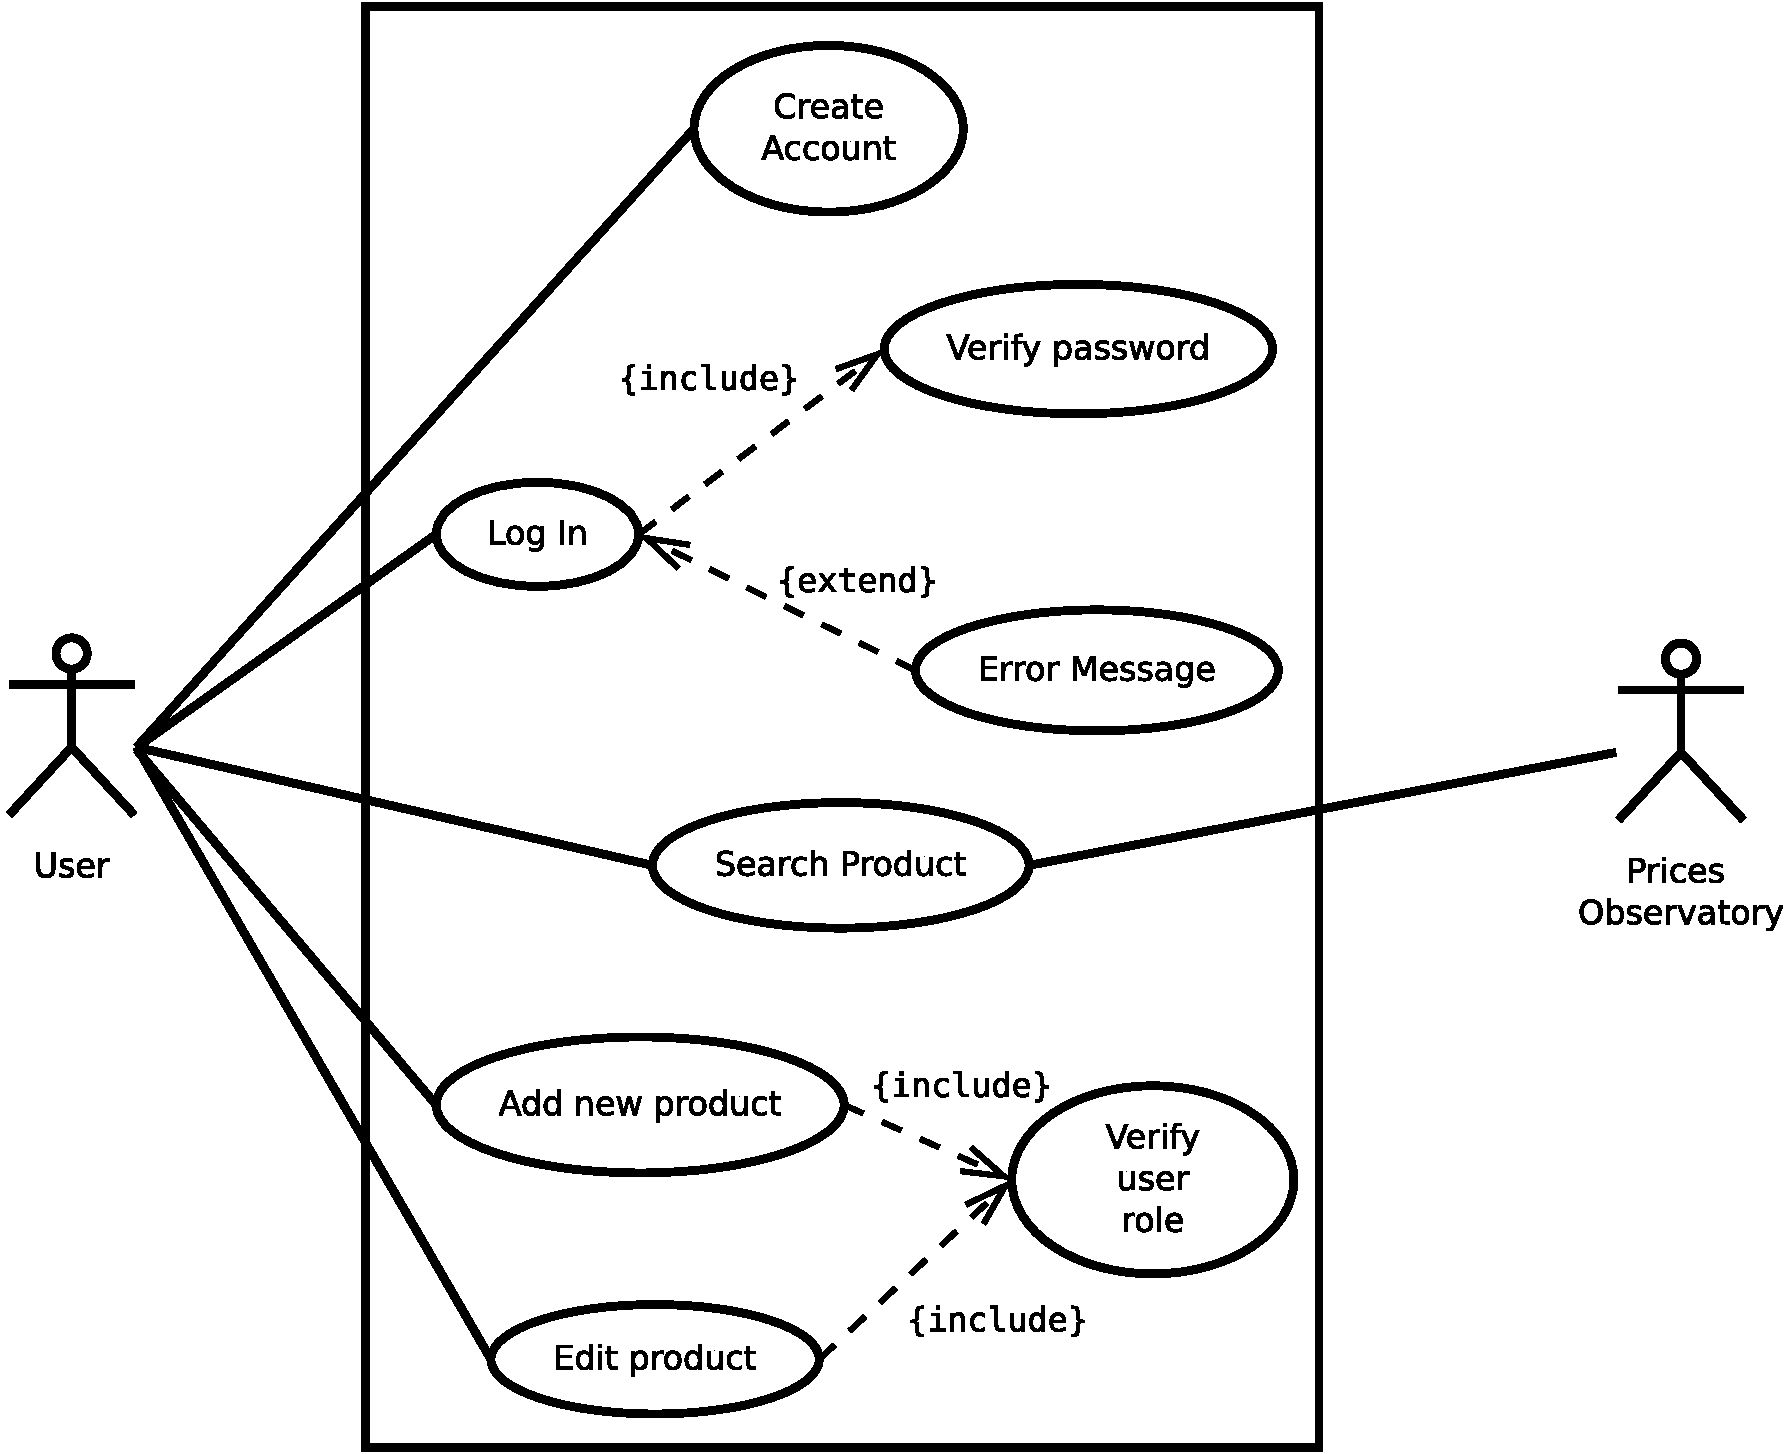
\includegraphics[scale=0.4,keepaspectratio=true]{./user_use_cases.pdf}
   \caption{Το use-case uml διάγραμμα της αλληλεπίδρασης του χρήστη με το παρατηρητήριο τιμών.}
    \label{uml1}
\end{figure}

\section{Αναφορές - πηγές πληροφοριών}
N/A

\section{Διαχειριστικές απαιτήσεις επιχειρησιακού περιβάλλοντος}

\subsection{Επιχειρησιακό μοντέλο}
N/A

\subsection{Περιβάλλον διαχείρισης πληροφοριών}
\hspace{0.6cm}Διαχείριση πληροφοριών είναι η συλλογή και διαχείριση πληροφορίας από διάφορες πηγές και η προσφορά της σε διάφορα κοινά. Ο όρος κοινό περιλαμβάνει τα εμπλεκόμενα μέρη της εφαρμογής διαχείρισης της πληροφορίας και οποιονδήποτε άλλο έχει δικαίωμα πρόσβασης σε αυτή. Ως διαχείριση ορίζεται η οργάνωση και ο έλεγχος στη δομή, την επεξεργασία και διανομή της πληροφορίας.

\hspace{0.6cm}Άρα η διαχείριση πληροφοριών επικεντρώνεται στην ικανότητα ενός οργανισμού να συλλέξει, διαχειριστεί, διατηρήσει, αποθηκεύσει και διανείμει τη σωστή πληροφορία στους σωστούς ανθρώπους, την κατάλληλη στιγμή.

\hspace{0.6cm}Με βάση τη σημερινή εικόνα η διαχείριση πληροφοριών πρέπει να υιοθετεί και να προσκολάτε στις εξής καθοδηγητικές αρχές:
\begin{itemize}
 \item Κάθε αντικείμενο πληροφορίας είναι περιουσιακό στοιχείο της εταιρείας στην οποία ανήκει η πλατφόρμα που το διατηρεί και διαχειρίζεται.
 \item Κάθε πληροφορία της πλατφόρμας πρέπει να είναι διαθέσιμη και να μοιράζεται. Προφανώς δεν γίνεται όλες οι πληροφορίες που διατηρεί η πλατφόρμα να είναι διαθέσιμες προς όλους, για παράδειγμα ευαίσθητες πληροφορίες χρηστών όπως τα passwords. Αλλά κατά γενικό κανόνα πρέπει οι γενικές πληροφορίες να είναι διαθέσιμες προς όλους γιατί προάγει την χρήση της πλατφόρμας και την εκμετάλευση επιχειρηματικής γνώσης.
 \item Η διαχείριση και διατήρησης κάθε πληροφορίας που πρέπει να κρατά πλατφόρμα γίνεται εταιρικά. Αποθηκεύεται και διατηρείται η πληροφορία, δηλαδή ό,τι προσθέτει ο χρήστης τη μία μέρα πρέπει να υπάρχει και την επόμενη.
\end{itemize}



\section{Λειτουργικές απαιτήσεις επιχειρησιακού περιβάλλοντος}

\subsection{Επιχειρησιακές διαδικασίες}
\hspace{0.6cm}Η επιχείρησή μας αποτελεί μία διαδικτυακή πλατφόρμα η οποία έχει σχεδιαστεί με σκοπό την προβολή και αγορά κινητών τηλεφώνων σε όσο το δυνατόν χαμηλότερες τιμές.

\hspace{0.6cm}Οι λειτουργικές απαιτήσεις της εφαρμογής μας, από τη μεριά των χρηστών-εθελοντών, είναι να υπάρχει η δυνατότητα καταχώρισης προϊόντος, καταστήματος, χρονικού και χωρικού αποτυπώματος όπως και καταχώριση της τιμής του προϊόντος-κινητού. 

\hspace{0.6cm}Επίσης παρέχουμε τη δυνατότητα να υπάρχουν ανώνυμοι χρήστες. Όσον αφορά αυτούς αλλά και τους χρήστες εθελοντές οι απαιτήσεις είναι να μπορούν να αναζητούν εύκολα και γρήγορα το εκάστοτε προϊόν που ψάχνουν και να λαμβάνουν για αυτό και κάποιες επιπρόσθετες πληροφορίες, όπως κάποιο γράφημα για την εξέλιξη της τιμής του ή τον αριθμό των καταστημάτων στα οποία υπάρχει διαθέσιμο, για κάποια συγκεκριμένη χρονική περίοδο.

\subsection{Περιορισμοί}

\hspace{0.6cm}Κανένας χρήστης δεν θα μπορεί να δει τους λογαριασμούς των άλλων χρηστών και επομένως δεν θα έχουν τη δυνατότητα ούτε να διαγράψουν κάποιον χρήστη ούτε να αλλάξουν το ρόλο του ούτε να αλλάξουν οποιοδήποτε στοιχείο των προσωπικών δεδομένων των υπολοίπων χρηστών. Επιπροσθέτως, κανένας χρήστης δεν θα μπορεί να διαγράψει προϊόντα ως οντότητες ούτε να αλλάξει στοιχεία τους πέρα από τα προβλεπόμενα. Δεν θα είναι δυνατή η εγγραφή χρηστών με ίδιο email ούτε με ίδιο username, διότι αυτά θα θεωρούνται μοναδικά από το σύστημα.

\hspace{0.6cm}Δεν θα είναι δυνατό να εμφανίζεται για κάποιο προϊόν το ίδιο κατάστημα πάνω από μία φορά με ίδια ή διαφορετική τιμή. Μετά την εισαγωγή νέων τιμών οι παλαιότερες τιμές δεν θα φαίνονται παρά μόνο σαν στατιστικό στοιχείο στον αντίστοιχο πίνακα.

\subsection{Δείκτες ποιότητας}
\hspace{0.6cm}Θα παρέχουμε ασφάλεια δεδομένων όπως και αξιόπιστο δίκτυο καθώς θα κάνουμε χρήση του πρωτοκόλλου HTTPS στην ιστοσελίδα μας. Άλλοι δείκτες ποιότητας είναι η ελάχιστη καθυστέρηση δικτύου (latency) για την ικανοποίηση μιας αίτησης, η συνέπεια των δεδομένων, η διαθεσιμότητα της εφαρμογής, η πιστοποίηση ταυτότητας του εθελοντή-χρήστη καθώς θα κάνει login με μοναδικό username και password, βάση δεδομένων.

\hspace{0.6cm}Τέλος το σύστημα μας θα είναι εύχρηστο διότι κάθε ενέργεια του χρήστη θα είναι πλήρως καθοδηγούμενη. Θα υπάρχουν ευδιάκριτα κουμπιά, πλήρως κατανοητά και κάθε τι που κάνει θα γίνεται με τρόπο που ενδεχομένως να γνωρίζει ήδη από αντίστοιχα συστήματα που έχει χρησιμοποιήσει στο παρελθόν.

\section{Έκθεση απαιτήσεων χρηστών}

\hspace{0.6cm}Η διαδικασία εξαγωγής και ανάλυσης των απαιτήσεων των χρηστών κατέληξε στις παρακάτω υψηλού επιπέδου απαιτήσεις που θα υλοποιεί το σύστημα:

\hspace{0.6cm}Οι χρήστες θέλουν να μπορούν να κάνουν αναζητήσεις για προϊόντα που τους ενδιαφέρουν και από τα αποτελέσματα της αναζήτησης να βλέπουν πληροφορίες για το προϊόν που θα επιλέγουν. Οι πληροφορίες αυτές πρέπει να είναι τα ονόματα των καταστημάτων στα οποία έχει καταγραφεί στο παρελθόν, η τελευταία τιμή η οποία έχει καταγραφεί για αυτά σε κάθε κατάστημα, η ημερομηνία και ώρα καταγραφής της τιμής καθώς και η διεύθυνση του καταστήματος σε κείμενο και σημείο στο χάρτη. 

\hspace{0.6cm}Άλλη απαίτηση είναι η προσθήκη νέων προϊόντων και τιμών καθώς και η ενημέρωση υπαρχόντων προϊόντων. Οι πληροφορίες που καταχωρούν θα είναι άμεσα διαθέσιμες σε όλους. Συνακόλουθα, προκειμένου να παρακολουθούν με γρήγορο και εύκολο τρόπο τα προϊόντα που τους ενδιαφέρουν, θα υπάρχει, ενδεχομένως, και μία λίστα αγαπημένων στο προφίλ τους.

\hspace{0.6cm}Εξίσου σημαντική απαίτηση των χρηστών, είναι η δυνατότητα να ειδοποιούνται για τυχόν πτώσεις τιμών ή για την διαθεσιμότητα (σε περίπτωση που κάποιο προϊόν δεν διατίθεται πλέον) των προϊόντων που έχουν συμπεριλάβει στη λίστα αγαπημένων τους. Ως εκ τούτου, η πλατφόρμα θα καλύπτει τις ανάγκες τους στο έπακρο, όσον αφορά την εξοικονόμηση χρόνου και χρημάτων.

\section{Αρχές του προτεινόμενου συστήματος}

\hspace{0.6cm}Το προτεινόμενο σύστημα θα έχει τις εξής λειτουργικές αρχές:
\newline
\begin{enumerate}
 \item Δυνατότητα δημιουργίας λογαριασμού χρήστη δίνοντας email, username και password.
 \item Δυνατότητα εισόδου ως χρήστης εισάγωντας τα email και password που ορίστηκαν κατά την εγγραφή του χρήστη.
 \item Δυνατότητα ανάκτησης password σε περίπτωση που ο χρήστης το ξέχασε.
 \item Δυνατότητα αναζήτησης προϊόντων με χρήση της μπάρας αναζήτησης που θα υπάρχει σε κάθε σελίδα που μπορεί να βρεθεί ο χρήστης.
 \item Λίστα αποτελεσμάτων αναζήτησης από όπου θα μπορεί ο χρήστης να επιλέξει όποιο προϊόν επιθυμεί.
 \item Μοναδικό προφίλ για κάθε προϊόν το οποίο θα περιλαμβάνει:
    \begin{enumerate}
     \item Όλα τα καταστήματα όπου είναι διαθέσιμο το προϊόν οργανωμένα σε δικούς τους <<τομείς>>.
     \item Η τελευταία τιμή η οποία καταγράφηκε για το αντίστοιχο κατάστημα.
     \item Η ημερομηνία καταχώρησης της τελευταίας τιμής.
     \item Η διεύθυνση του αντίστοιχου καταστήματος.
     \item Χάρτης όπου θα φαίνεται το στίγμα της τοποθεσίας του καταστήματος.
     \item Κουμπί επεξεργασίας δίπλα σε κάθε κατάστημα για προσθήκη νέας τιμής.
     \item Κουμπί για προσθήκη νέου καταστήματος.
     \item Πίνακας με στατιστικά στοιχεία της διακύμανσης της τιμής.
    \end{enumerate}
\item Δυνατότητα προσθήκης νέου προϊόντος μέσω αντίστοιχου κουμπιού που οδηγεί σε φόρμα εισαγωγής στοιχείων του προϊόντος, όπου θα ζητηθούν τα εξής:
    \begin{enumerate}
     \item Μήνυμα ενεργοποίησης gps εφόσον ο χρήστης το επιθυμεί.
     \item Δεδομένου ότι το gps είναι ενεργό τότε θα εντοπίζεται η τοποθεσία του χρήστη και θα συμπληρώνεται η διεύθυνση του καταστήματος.
     \item Εισαγωγή ονόματος προϊόντος.
     \item Εισαγωγή ονόματος καταστήματος.
     \item Εισαγωγή τιμής σε \texteuro.
     \item Εισαγωγή διεύθυνσης καταστήματος αν ο χρήστης δεν επιλέξει να ενεργοποιήσει το gps της συσκευής του.     
    \end{enumerate}
\item Το χρονικό αποτύπωμα του χρήστη θα λαμβάνεται σε όλες τις περιπτώσεις αυτόματα από το ρολόι του συστήματος της συσκευής του.
\item Διατήρηση λίστας για κάθε χρήστη αγαπημένων προϊόντων στην οποία θα μπορεί να προσθέτει και να αφαιρεί όποιο προϊόν θέλει.
\item Δυνατότητα αποσύνδεσης.
\end{enumerate}

\vspace{0.5cm}
\textbf{Σενάριο 1-Αποτυχημένη αναζήτηση προϊόντος}\\
\begin{enumerate}
 \item Ο  ανώνυμος χρήστης ανοίγει την αρχική σελίδα και πληκτρολογεί το όνομα του προϊόντος στην μπάρα αναζήτησης.
 \item Το αντικείμενο δεν βρέθηκε και εμφανίζεται μήνυμα αποτυχίας με δυνατότητα αναζήτησης νέου προϊόντος.
\end{enumerate}

\vspace{0.5cm}
\textbf{Σενάριο 2-Επιτυχημένη αναζήτηση προϊόντος}\\
\begin{enumerate}
 \item Ο  ανώνυμος χρήστης ανοίγει την αρχική σελίδα και πληκτρολογεί το όνομα του προϊόντος στην μπάρα αναζήτησης.
 \item Το αντικείμενο βρέθηκε και εμφανίζονται τα μαγαζιά στα οποία υπάρχει και οι αντίστοιχες τιμές που έχει κάθε κατάστημα.
\end{enumerate}

\vspace{0.5cm}
\textbf{Σενάριο 3-Προσθήκη καινούργιας τιμής-καταστήματος σε υπάρχον προϊόν}\\
\begin{enumerate}
 \item Ο χρήστης ανοίγει την αρχική σελίδα και πληκτρολογεί το όνομα του προϊόντος στην μπάρα αναζητήσης.
 \item Το αντικείμενο βρέθηκε και εμφανίζονται τα μαγαζιά στα οποία υπάρχει και οι αντίστοιχες τιμές που έχει κάθε κατάστημα.
 \item Μπορεί να τροποποιήσει την τιμή που έχει το προϊόν σε κάποιο κατάστημα μέσω αντίστοιχου κουμπιού επεξεργασίας της τιμής ή να προσθέσει καινούργιο κατάστημα το οποίο δεν είναι καταχωρημένο ότι παρέχει το προϊόν, μέσω κουμπιού προσθήκης προϊόντος.
 \item Αν ο χρήστης δεν είναι συνδεδεμένος ήδη το πάτημα ενός εκ των δύο κουμπιών ρωτάει τον χρήστη αν έχει λογαριασμό ή αν επιθυμεί να δημιουργήσει στην περίπτωση που δεν διαθέτει.
 \begin{itemize}
  \item Ο ήδη εγγεγραμμένος χρήστης συμπληρώνει το email και το password του.
  \item Αν ο εγγεγραμμένος χρήστης εισάγει λάθος password εμφανίζεται μήνυμα αποτυχίας και του δίνεται η  δυνατότητα να ξανά εισάγει το password ή να πατήσει ότι το ξέχασε και να εκκινήσει διαδικασία ανάκτησης.
  \item O μη εγγεγραμμένος συμπληρώνει σε διπλανή φόρμα το email, username και κάποιο password που επιθυμεί.
 \end{itemize}

 \item  Επιτυχής σύνδεση οδηγεί σε φόρμα προσθήκης νέου προϊόντος όπου ο χρήστης συμπληρώνει το όνομα του, το όνομα του καταστήματος και την τιμή του, στην περίπτωση εισαγωγής προϊόντος σε κατάστημα που δεν υπάρχει καταχωρημένο. Αλλιώς, του εμφανίζεται η υπάρχουσα τιμή του προϊόντος σε συγκεκριμένο κατάστημα με δυνατότητα επεξεργασίας της τιμής.
 
 \item Εφόσον ο χρήστης το επιθυμεί, ανοίγοντας το gps του λαμβάνεται αυτόματα η τοποθεσία του ως διεύθυνση του καταστήματος, στην περίπτωση εισαγωγής προϊόντος σε κατάστημα που δεν υπάρχει καταχωρημένο.
 \item Πατώντας το κουμπί αποθήκευσης ο χρήστης οδηγείτε στο προφίλ του προϊόντος όπου φαίνεται η νέα καταχώρηση καταστήματος-τιμής ή η νέα-ανανεωμένη τιμή του προϊόντος σε υπάρχον κατάστημα, η ημερομηνία και ώρα καταχώρησης, τις οποίες πρόσθεσε το σύστημα αυτόματα από τη συσκευή του χρήστη, και ο χάρτης με την τοποθεσία του καταστήματος. 
\end{enumerate}

\vspace{0.5cm}
\textbf{Σενάριο 4-Προσθήκη νέου προϊόντος}\\
\begin{enumerate}
 \item Ο χρήστης ανοίγει την αρχική σελίδα και πληκτρολογεί το όνομα του προϊόντος στην μπάρα αναζητήσης.
 \item Το αντικείμενο δεν βρέθηκε και εμφανίζεται μήνυμα αποτυχίας και η επιλογή μέσω κουμπιού προσθήκης νέου προϊόντος
 \item Αν ο χρήστης δεν είναι συνδεδεμένος ήδη το πάτημα του κουμπιού ρωτάει τον χρήστη αν έχει λογαριασμό ή αν επιθυμεί να δημιουργήσει στην περίπτωση που δεν διαθέτει.
 \begin{itemize}
  \item Ο ήδη εγγεγραμμένος χρήστης συμπληρώνει το email και το password του.
  \item Αν ο εγγεγραμμένος χρήστης εισάγει λάθος password εμφανίζεται μήνυμα αποτυχίας και του δίνεται η  δυνατότητα να ξανά εισάγει το password ή να πατήσει ότι το ξέχασε και να εκκινήσει διαδικασία ανάκτησης.
  \item O μη εγγεγραμμένος συμπληρώνει σε διπλανή φόρμα το email, username και κάποιο password που επιθυμεί.
 \end{itemize}
 \item Επιτυχής σύνδεση οδηγεί σε φόρμα προσθήκης νέου προϊόντος όπου ο χρήστης συμπληρώνει το όνομα του, το όνομα του καταστήματος και την τιμή του.
 \item Εφόσον ο χρήστης το επιθυμεί και ανοίγοντας το gps του λαμβάνεται αυτόματα η τοποθεσία του ως διεύθυνση του καταστήματος. Αλλιώς την εισάγει με το χέρι.
 \item Πατώντας το κουμπί αποθήκευσης ο χρήστης οδηγείτε στο προφίλ του προϊόντος όπου φαίνεται η νέα καταχώρηση καταστήματος-τιμής, η ημερομηνία και ώρα καταχώρησης, τις οποίες πρόσθεσε το σύστημα αυτόματα από τη συσκευή του χρήστη, και ο χάρτης με την τοποθεσία του καταστήματος.
\end{enumerate}


\section{Περιορισμοί στο πλαίσιο του έργου}
N/A

\section{Παράρτημα: ακρωνύμια και συντομογραφίες}
N/A



\end{document}
